% Use class option [extendedabs] to prepare the 1-page extended abstract.
\documentclass[extendedabs]{bmvc2k}

\begin{document}

\title{Project \texttt{MATRIX} : On-set 3D Reconstruction Tool }

\addauthor{Louis Viot}{louis.viot@etu.enseeiht.fr}{1}

\addinstitution{
Department of Applied Mathematics and Computer Science,\\
 ENSEEIHT}
\maketitle
\noindent
\textbf{Keywords} : \textit{VORTEX, Mikros Image~\cite{mikros}, POPART, MATRIX, On-set 3D Reconstruction Tool, 3D, openMVG, Cinema, CGI, Reconstruction}

\section*{Abstract}
Ce rapport a pour but de résumer notre impression sur ce début de projet long. Notamment ce que l'on ressent par rapport, non pas au développement même d'un point de vu logiciel du projet, à la gestion de projet. Nous aborderons dans ce rapport différents points en rapport au cours de gestion de projet et appliqués à ce projet long. On abordera rapidement mon impression par rapport à l'organisation de l'équipe, la plannification, la gestion des risques et la gestion des réunions.\vspace{3cm}
\subsubsection*{Versions}
\noindent
\texttt{version 0.1} : rédaction du corp du rapport \\
\texttt{version 0.2} : intégration des images \\
\texttt{version 0.9} : traduction en \LaTeX \\
\texttt{version 1.0} : relecture et version finale

\section{Context}
Dans un réacteur nucléaire se trouve le coeur constitué de crayons de combustible (principalement de plutonium et d'uranium). Ces crayons sont assemblés à l'aide de gaines et sont placés dans le réacteur. Un circuit complexe d'eau est ensuite installé et permet de faire passer l'eau à l'intérieur de ces gaines. La réaction de fission de l'uranium et du plutonium va provoquer l'émission de particules hautement énergétiques qui vont chauffer l'eau dans le circuit. L'eau va ensuite passer dans un pressuriseur et se transformera en vapeur qui fera tourner plusieurs turbines, ce qui va provoquer la production d'électricité (voir figure~\ref{reacteur}). Le fonctionnement d'un 
réacteur nucléaire est bien sur bien plus complexe que cela, mais dans le cadre du stage, le fonctionnement en détail du réacteur n'a pas besoin d'être connu, le principal étant de comprendre qu'à l'intérieur du coeur du réacteur se trouve des crayons de combustible, et que ce sont ces crayons qui vont pouvoir provoquer les accidents graves.\\

\begin{figure}[h]
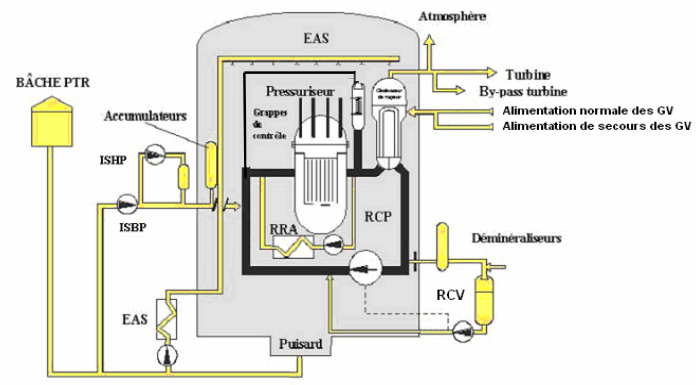
\includegraphics[scale=0.5]{reacteur.png}
\caption{Schéma d'un réacteur nucléaire}
\label{reacteur}
\end{figure}


Un crayon est formé de combustible (uranium et plutonium), mais aussi d'une gaine en Zirconium pour maintenir les pastilles de combustible ensemble. Un accident grave est généralement causé par un problème de refroidissement de ces crayons de combustible dont la puissance résiduelle ne pourra plus être efficacement évacuée. Ces crayons vont alors fondre et former un mélange appelé corium principalement formé de zirconium, d'uranium,de plutonium et parfois de nickel et de chrome venant des installations. La température peut dépasser les 2800K. L'étude de ce mélange est centrale dans l'approche des accidents graves : du fait de sa forte teneur en élément radioactif, ce mélange est destructeur et la propagation de ce mélange peut être fatale à toute l'installation. Le corium se propage alors dans la cuve, puis s'il détruit la cuve, se propage dans le bâtiment du réacteur, et, encore plus grave,à l'éxtérieur du réacteur s'il détruit la structure généralement en béton de celui-ci. Ainsi, en se propageant, le corium réagit avec les différents éléments du réacteur et plusieurs types d'intéraction peuvent alors se produire : intéraction avec l'eau froide du réacteur (ICE), ou encore intéraction avec le béton du fond du réacteur (ICB).  Lorsque le corium commence à se propager dans le réacteur, il y a ainsi de forte chance pour que le réacteur ne puisse plus jamais fonctionner, le but n'est donc pas d'essayer de sauvegarder le réacteur mais de prévenir toute perte humaine. \\

Dans le domaine des accidents graves, les phénomènes physiques mis en jeu sont trés complexes et ne peuvent être bien étudiés à l'heure actuelle. La but de l'étude des accidents graves est de comprendre au mieux ces 
phénomènes, de produire des codes de simulation qui pourront prévoir, toujours au mieux, le comportement du corium mais aussi et sutout d'essayer de majorer l'erreur comise lors de telles simulations. Comme dit précédemment,
les données concernant les accidents graves sont actuellement trés limitées et il est trés difficile de produite de nouvelles données. On peut récupérer des données de prédents accidents (Three Mile Island, Fukushima, Tchernobyl),
ou encore faire des simulations à échelle réduite (installation PLINIUS au Cea Cadarache par exemple). Les codes scénario permettent ainsi de simuler la propagation du corium au sein de l'enceinte du réacteur. Le code PROCOR 
est le code développé au laboratoire LPMA du Cea Cadarache où se déroule le stage. C'est un code orienté objet en Java permettant de créer des applications PROCOR prenant différents modèles (comme un modèle de cuve, un modèle 
de corium) et permettant de simuler les intéractions entre ces modèles. Ainsi une application PROCOR prend la forme d'un système dynamique qui évolue au cours du temps, ce système dynamique étant composé de plusieurs modèles
et d'un ensemble d'intéraction entre ces modèles. Chaque modèle peut évoluer pendant le cycle de vie de l'application, il peut être détruit si par exemple un élément comme le corium détruit une enceinte. La plateforme permet,
 par le biais de méthodes de Monte-Carlo d'obtenir des probabilités de rupture de cuve, ou plus généralement permet d'avoir des résultats de sensibilité sur certain paramètre physique et d'incertitude sur certains matériaux.  

\section{Difficulties and Choices}
First of all, before even thinking about programming language, we had to think of a solid and re-usable architecture for
our application. Because we had to build a GUI that would launch openMVG executable, we quickly choose to use the 
model/view/controller pattern. This pattern is pretty simple to understand : the user uses a controller which will manipulate
the model which will update the view that the user sees. In our context, the model correspond to the openMVG executables for example. 
What we actually choose was to modify a bit this pattern to perfectly fit our needs : we would merge the controller and view
together, we will explain later why.

Once we had built a solid architecture, and that the client confirm the architecture was what he needed, we thought about 
programming languages. We firstly choose to use C++ for the model code for two reasons : because nobody knew at this time 
how to use this language and because it is a very powerful and low level language. To create the GUI, we choose to use Qt, which
is a "cross-platform application for developpers using C++"  according to their website, so that it perfectly fits our needs. But later in
the project, the client told us that he would rather us to use Python instead of C++. Python was also a challenge for us because no one knew it at 
this time. After choosing python, we had to restart almost everything, forget what we learned and start over. That was a important milestone in our
project. We choose to stay with Qt and QML for the GUI, but we had to adapt it in order to make it work with Python : that's why we used PyQt, a "binding" between
Qt, coded to use with C++, and Python, that allows us to communicate between Python et Qt. 

When we were set on the programming languages, we did a prototype of our application to test communication between the model, in python, and the view/controller, in PyQt and QML. 
The power of PyQt and Python is the communication in signal/slot : one can emit signal in a module and another module can receive this signal in it's slot. So module, in PyQt or Python, 
can exchange any objects through this system. Throughout the project, we always kept in mind that our goal was to build a easily re-usable application. That's why we used the architecture described
above but adapted to the signal/slot communication (see figure~\ref{arch}) : only two "modules", the orchestrator and the main window, can communicate in our application so that whenever a developper wants
to add a GUI or a model module, he only has to connect it to the orchestrator or the main window. Modules are then connected to either the orchestrator or the main window, and they handle the communication. 
\begin{figure}[t]
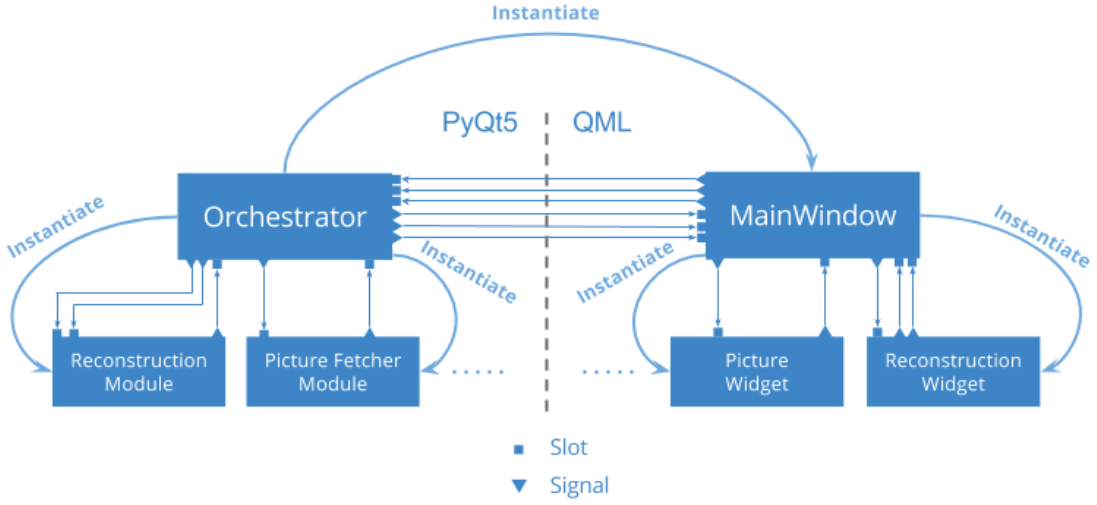
\includegraphics[width=\linewidth]{images/arch.png}
\caption{Architecture of the application (\texttt{PyQt5} for the model, \texttt{QML} for the view)}
\label{arch}
\vspace{-2mm}
\end{figure}


The last really important milestone we had was the 3D renderer : because python is more high level than C++, there are not really any optimised openGL libraries for python. But one important application requirement
was a performant renderer to render big point clouds. So instead of using openGL with python, we used openGL with C++ and then we created a QML plugin to import in PyQt. Though we first thought that this was a huge 
problem, it turns out to be a really good example on how our application was highly cutomizable and modular : one can easily import plugin coded in any language they want as long as they convert it into QML plugin. 

\section{Results and possible improvements}
Results are really satisfying given the fact that we knew absolutely none of the languages we used at the beginning and that the application is supposed to be a prototype. We ended up having more than 7000
lines of code in the languages described previously. There are still a few improvements to be made 
but for the moment one can import pictures from either his camera or his computer, sort them, delete them, launch a 3D recontruction on those images, and then see the result on the renderer and see cameras positions on a map.
We also implement interaction between the map and the photo list : if a user click on a picture, it will center the map on the GPS position of the camera used to take this picture. The user can also manage a workspace, even multiple workspaces, in which he can add scenes. One scene has one or multiple pictures, and it is from one scene that the user can launch a 3D reconstruction. The application comes with installation instructions and even a documentation (see ~\cite{doc}). To conclude on those results, we have, at the end of this project, a pretty good prototype and our clients were pretty satisfied with the result. Here is a screenshot of the application :
\begin{figure}[t]
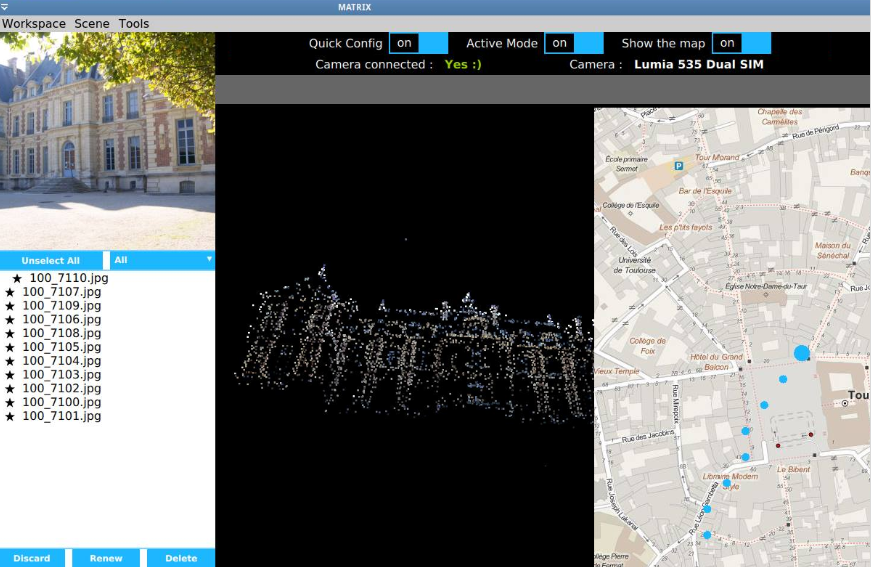
\includegraphics[width=\linewidth]{images/app.png}
\caption{Screenshot of the final application}
\label{app}
\vspace{-2mm}
\end{figure}

In further version, we could add the same type of interaction between the 3D renderer and the photo list. We could also launch the reconstruction in another thread to not block the entire application while a reconstruction is processed.

\bibliography{egbib}
\end{document}





